\subsection{Paquete 7: Mensajería contextual}

    El canal de mensajería vincula cada hilo de chat con el anuncio correspondiente. Permite que inquilinos y propietarios intercambien mensajes antes o después de reservar, manteniendo el histórico de comunicaciones, el estado de lectura y la trazabilidad necesaria ante disputas. La figura \ref{fig:dcu_mensajeria} esquematiza los cinco casos de uso del módulo (CU64 a CU68).

\begin{figure}[H]
    \centering
    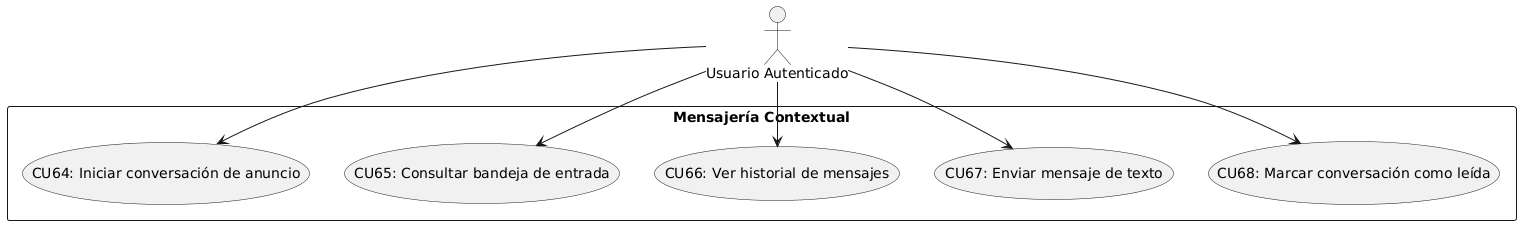
\includegraphics[width=0.75\textwidth]{AnalisisFuncional/img/dcu_mensajeria.png}
    \caption{Diagrama de casos de uso de mensajería contextual}
    \label{fig:dcu_mensajeria}
\end{figure}

    Las siguientes tablas recogen la especificación de CU64 a CU68:

\begin{table}[H]
\centering
\begin{tabular}{|p{3.2cm}|p{11.3cm}|}
\hline
\textbf{Caso de Uso} & \textbf{CU64: Iniciar conversación vinculada a un anuncio} \\ \hline
\textbf{Actores} & Usuario Autenticado \\ \hline
\textbf{Descripción} & Abre un nuevo hilo de chat directo entre el usuario y el anfitrión de una publicación \\ \hline
\textbf{Precondiciones} & Estar autenticado, que el anuncio esté activo y no ser el propio propietario del mismo \\ \hline
\textbf{Flujo básico} & 
1. El usuario accede a la ficha de un alojamiento y pulsa sobre la opción de contactar. \newline
2. El sistema comprueba si ya existía una conversación previa abierta para ese contexto. \newline
3. Si existe, redirige al hilo histórico; en caso contrario, inicializa un nuevo canal vinculado. \newline
4. La interfaz abre la ventana de conversación lista para la redacción de mensajes. \\ \hline
\end{tabular}
\caption{Especificación del caso de uso CU64}
\label{tab:cu64}
\end{table}

\begin{table}[H]
\centering
\begin{tabular}{|p{3.2cm}|p{11.3cm}|}
\hline
\textbf{Caso de Uso} & \textbf{CU65: Consultar bandeja de entrada y no leídos} \\ \hline
\textbf{Actores} & Usuario Autenticado \\ \hline
\textbf{Descripción} & Despliega la relación de hilos de mensajería del usuario con indicadores de mensajes pendientes \\ \hline
\textbf{Precondiciones} & Mantener una sesión autenticada activa \\ \hline
\textbf{Flujo básico} & 
1. El usuario accede a la sección de mensajes desde la barra superior de navegación. \newline
2. El sistema recupera las conversaciones activas ordenadas por la fecha del último mensaje. \newline
3. La interfaz presenta los resúmenes de cada chat, los avatares y el recuento de no leídos. \\ \hline
\end{tabular}
\caption{Especificación del caso de uso CU65}
\label{tab:cu65}
\end{table}

\begin{table}[H]
\centering
\begin{tabular}{|p{3.2cm}|p{11.3cm}|}
\hline
\textbf{Caso de Uso} & \textbf{CU66: Ver historial de mensajes} \\ \hline
\textbf{Actores} & Usuario Autenticado \\ \hline
\textbf{Descripción} & Carga y visualiza la secuencia cronológica de intervenciones dentro de una conversación \\ \hline
\textbf{Precondiciones} & Ser participante legítimo (emisor o receptor) de la conversación seleccionada \\ \hline
\textbf{Flujo básico} & 
1. El usuario selecciona un hilo de conversación de su bandeja de entrada. \newline
2. El backend verifica la pertenencia del usuario al hilo solicitado. \newline
3. El sistema devuelve los mensajes paginados con sus marcas de tiempo asociadas. \newline
4. La interfaz renderiza el diálogo diferenciando visualmente los mensajes propios y ajenos. \\ \hline
\end{tabular}
\caption{Especificación del caso de uso CU66}
\label{tab:cu66}
\end{table}

\begin{table}[H]
\centering
\begin{tabular}{|p{3.2cm}|p{11.3cm}|}
\hline
\textbf{Caso de Uso} & \textbf{CU67: Enviar mensaje de texto} \\ \hline
\textbf{Actores} & Usuario Autenticado \\ \hline
\textbf{Descripción} & Transmite un nuevo mensaje de texto plano hacia el destinatario en el hilo activo \\ \hline
\textbf{Precondiciones} & Formar parte de la conversación y que el contenido no supere los límites de longitud \\ \hline
\textbf{Flujo básico} & 
1. El usuario introduce el texto en el área de entrada del chat y pulsa enviar. \newline
2. El cliente valida que el cuerpo del mensaje no se encuentre vacío. \newline
3. El backend persiste el mensaje en base de datos con la marca temporal actual. \newline
4. El sistema notifica al receptor y actualiza la vista de la conversación en tiempo real. \\ \hline
\end{tabular}
\caption{Especificación del caso de uso CU67}
\label{tab:cu67}
\end{table}

\begin{table}[H]
\centering
\begin{tabular}{|p{3.2cm}|p{11.3cm}|}
\hline
\textbf{Caso de Uso} & \textbf{CU68: Marcar conversación como leída} \\ \hline
\textbf{Actores} & Usuario Autenticado \\ \hline
\textbf{Descripción} & Actualiza el estado de los mensajes entrantes poniendo a cero los indicadores pendientes \\ \hline
\textbf{Precondiciones} & Tener mensajes recibidos no leídos en el hilo visualizado \\ \hline
\textbf{Flujo básico} & 
1. El usuario abre o mantiene en foco una conversación con mensajes pendientes. \newline
2. El cliente emite una petición asíncrona informando de la visualización del hilo. \newline
3. El backend actualiza la marca de lectura de los mensajes correspondientes. \newline
4. La interfaz disminuye o suprime los distintivos numéricos de notificación global. \\ \hline
\end{tabular}
\caption{Especificación del caso de uso CU68}
\label{tab:cu68}
\end{table}